\documentclass{article}

\usepackage{graphicx} % Required for inserting images
\usepackage{mathtools}
\usepackage[hidelinks]{hyperref}
%\usepackage{bbm}  % for \mathbb and \mathbbm symbols
\usepackage{amsmath,amsfonts,amssymb, amsthm}
\usepackage{cleveref} % this needs to go after hyperref and amsmath

%\usepackage[chapter]{algorithm}  % for algorithm environment, option: use chapters for numering
\usepackage{tikz}
\usetikzlibrary{positioning}

\usepackage{tikz-cd}  % commuting diagrams based on tikz
\usetikzlibrary{calc}
\usetikzlibrary{external}
\usepackage{booktabs}  % for clean tables (tabular environment) 
\usepackage{caption}  % for setting caption width
\captionsetup{width=\linewidth}

\usepackage[textsize=tiny]{todonotes} % For todos (check opencompl template if more is necessary)

\usepackage{tablefootnote}   %
\usepackage{tabularx}        %

\definecolor{Green}{rgb}{0, 0.5, 0.2}
\usepackage[dvipsnames,table]{xcolor}
\usetikzlibrary{decorations.markings}
\usepackage{float}
\usepackage{makecell} % for tables
\usepackage{pifont}
\usepackage{multicol}

\usepackage{pdflscape} % https://www.namsu.de/Extra/befehle/Querformat.html

\usepackage{circledsteps} % for \Circled

\usepackage{longtable, array} % for the notation table



\usepackage{titlesec}
\titleformat{\chapter}[display]
  {\normalfont\huge\scshape}
  {\thechapter}
  {0.5em}
  {}
  [\vspace{0.5ex}\titlerule]

% Section
\titleformat{\section}
  {\normalfont\Large\scshape}
  {\thesection}
  {0.5em}
  {}

% Subsection
\titleformat{\subsection}
  {\normalfont\large}
  {\thesubsection}
  {0.5em}
  {}

\captionsetup{width=\textwidth, labelfont=bf, font=small}

\definecolor{greenii}{RGB}{20,140,10}
\definecolor{darkgreen}{rgb}{0.00,0.85,0.1}

\newcommand{\red}[1]{{\color{red} {#1}}}
\newcommand{\orange}[1]{{\color{orange} {#1}}}
\newcommand{\blue}[1]{{\color{blue} {#1}}}
\newcommand{\green}[1]{{\color{OliveGreen} {#1}}}

\usepackage[backend=biber, maxbibnames=3,style=alphabetic , backref,backrefstyle=none]{biblatex}
\addbibresource{bachelors.bib}

\AtEveryBibitem{
  \clearfield{issn}
  \clearfield{language}
  \clearfield{note}
  \clearfield{urldate}
}

\AtEveryBibitem{%
  \ifboolexpr{
    ( test {\ifentrytype{article}} or test {\ifentrytype{online}})
    and
    ( not test {\iffieldundef{doi}} or not test {\iffieldundef{eprint}} )
  }
  {\clearfield{url}}
  {}
}

\AtEveryBibitem{%
  \ifboolexpr{
    not test {\iffieldundef{doi}}
    or not test {\iffieldundef{eprint}}
  }
  {\clearfield{url}}
  {}
}

\newcommand{\ket}[1]{\ensuremath{\left| #1 \right\rangle}}
\newcommand{\bra}[1]{\ensuremath{\left\langle #1 \right|}}
\newcommand{\braket}[2]{\ensuremath{\left\langle #1 \middle| #2 \right\rangle}}
\newcommand{\ketbra}[2]{\ensuremath{\left| #1 \right\rangle \left\langle #2 \right|}}
\newcommand{\braopket}[3]{\ensuremath{\left\langle #1 \middle| #2 \middle| #3 \right\rangle}}

\newcommand{\SU}[1]{\mathrm{SU}(#1)}
\newcommand{\SO}[1]{\mathrm{SO}(#1)}
\newcommand{\U}[1]{\mathrm{U}(#1)}
\newcommand{\Sp}[1]{\mathrm{Sp}(#1)}
\newcommand{\GL}[1]{\mathrm{GL}(#1)} % e.g., GL(n, R)
\newcommand{\SL}[2]{\mathrm{SL}(#1, #2)}

\newcommand{\liesl}[1]{\mathfrak{sl}_{#1}} % sl_2 lie algebra.

%\theoremstyle{italics}
\newtheorem{theorem}{Theorem}[section]
\newtheorem{lemma}[theorem]{Lemma}
\newtheorem{fact}[theorem]{Fact}
\newtheorem{conjecture}[theorem]{Conjecture}
\newtheorem{proposition}[theorem]{Proposition}
\newtheorem{corollary}[theorem]{Corollary}
\theoremstyle{definition}
\newtheorem{definition}[theorem]{Definition}
\newtheorem{graphicalCalculus}[theorem]{Graphical Notation}
\newtheorem{notation}[theorem]{Notation}
\newtheorem{literature}[theorem]{Literature}
\newtheorem{example}[theorem]{Example}
\newtheorem{assumption}[theorem]{Assumption}
\newtheorem{examples}[theorem]{Examples}
\newtheorem{remark}[theorem]{Remark}
%\newtheorem{proof}{Proof}

\newcommand{\Cat}{\mathbf{Cat}}          % Category of categories
%\newcommand{\VecCat}{\mathbf{Vect}}      % Category of Vector spaces
\newcommand{\Veck}{\mathrm{fdVect_k}}
\newcommand{\Rep}{\mathrm{Rep}}          % Representation category
\newcommand{\Hom}{\operatorname{Hom}}    % 
\newcommand{\End}{\operatorname{End}}    % Endomorphism set
\newcommand{\id}{\operatorname{id}}      % Identity morphism
\newcommand{\Hilb}{\operatorname{fdHilb}}
\newcommand{\del}{\boxtimes}
\newcommand{\sVect}{\mathrm{sVect}}
\newcommand{\gVSpace}[1]{\mathrm{Vec}_{#1}} % Graded Vector Space
\newcommand{\Fib}{\mathrm{Fib}}
\newcommand{\Set}{\mathrm{Set}}
\newcommand{\sgotimes}[1]{\otimes_{\scriptscriptstyle#1}} % small Graded Tensor Space
\newcommand{\gotimes}[1]{\otimes_{#1}} % G-graded vectors space 
\newcommand{\ot}{\otimes}
\newcommand{\op}{\oplus}
\newcommand{\bop}{\bigoplus}
\newcommand{\bigot}{\bigotimes}
\newcommand{\kot}{\otimes^k}
\newcommand{\iot}{\otimes} % placeholder for isotypic tensoring
\newcommand{\overeq}[1]{\overset{#1}{=}} % move
\newcommand{\ob}{\mathrm{ob}} % \ob of the category
\newcommand{\Irr}{\mathrm{Irr}} % Irreps of the category
\newcommand{\uConf}{\mathrm{Conf}} % Unordered ConfigurationSpace
\newcommand{\oConf}[1]{\underset{\{1, \ldots, #1\}}{\uConf}}
\newcommand{\Br}{\mathrm{Br}} % Braid Group
\newcommand{\PBr}{\mathrm{PBr}} % Pure braid group

\newcommand{\Hilbfd}{\mathrm{Hilb_{\text{fd}}}}

\newcommand{\Mod}[1]{\operatorname{Mod}_{#1}}

\newcommand{\FDVec}[1]{\mathrm{FD}#1\mathrm{Vec}}
\newcommand{\VecCat}[1]{\mathrm{Vec}_#1}

\newcommand{\Z}{\mathbb{Z}}
\newcommand{\C}{\mathbb{C}}
\newcommand{\R}{\mathbb{R}}

\newcommand{\CC}{\mathcal{C}}
\newcommand{\CD}{\mathcal{D}}

\newcommand{\ev}{\operatorname{ev}}
\newcommand{\coev}{\operatorname{coev}}
\newcommand{\tr}{\operatorname{tr}}
\newcommand{\Mat}[3]{\mathrm{Mat}_{#1 \times #2}(#3)}



\makeatletter
\definecolor{RoyalBlue}{HTML}{4169E1}
\definecolor{CiteViolet}{HTML}{7B2CBF}
\hypersetup{
    colorlinks=true,
		linkcolor=Maroon,
    %linkcolor = CiteViolet,
		citecolor=RoyalBlue,
    urlcolor=RoyalBlue
}
\makeatother


\definecolor{purple}{rgb}{0.6, 0.1, 0.6}
\definecolor{darkgreen}{rgb}{0.1, 0.5, 0.1}
\definecolor{darkblue}{rgb}{0.1, 0.2, 0.7}

% ==========================================
% Quantum Circuit Macros
% ==========================================

% \drawGate{x}{y}{Label}
\newcommand{\drawGate}[3]{
  \node[draw, fill=white, line width=1pt, minimum width=0.7cm, minimum height=0.7cm] at (#1, #2) {$#3$};
}

% \drawCNOT{x}{y_control}{y_drop}
% Draws a CNOT gate. The target is located at y_control - y_drop.
\newcommand{\drawCNOT}[3]{
  \draw[line width=1pt] (#1, #2) -- (#1, #2 - #3);
  % Control dot
  \filldraw[black] (#1, #2) circle (2.5pt);
  \draw[line width=1pt, fill=white] (#1, #2 - #3) circle (4pt);
  \draw[line width=1pt] (#1-4pt, #2 - #3) -- (#1+4pt, #2 - #3);
  \draw[line width=1pt] (#1, #2 - #3 - 4pt) -- (#1, #2 - #3 + 4pt);
}

% \drawMeasurement{x}{y}
\newcommand{\drawMeasurement}[2]{
  \node[draw, fill=white, line width=1pt, minimum width=0.8cm, minimum height=0.6cm] at (#1, #2) {};
  \draw[line width=0.8pt] (#1-0.25, #2-0.1) arc (180:0:0.25);
  \draw[line width=0.8pt, ->] (#1, #2-0.1) -- (#1+0.2, #2+0.2);
}

% \drawControlledGate{x}{target_y}{Label}{control_y}
\newcommand{\drawControlledGate}[4]{
  \drawGate{#1}{#2}{#3}
}

% ======
% Braid Macros

% \drawInjectionWeave{x}{y}{Label}{a}{b}{c}
\newcommand{\drawInjectionWeave}[6]{
  \node[draw, fill=white, line width=1pt, minimum width=0.7cm, minimum height=0.7cm] at (#1, #2) {$#3$};
}

\usepackage{libertine}
\usepackage[libertine]{newtxmath}
\renewcommand{\ttdefault}{cmtt}

\tikzset{
    fusionarrow/.style={
        postaction={
            decorate,
            decoration={
                markings,
                mark=at position 0.55 with {\arrow[scale=1.0]{Stealth}}
            }
        }
    }
}

% Left-aligned 3-label fusion tree
\newcommand{\FusionTreeThreeLabel}[5]{%
\begin{tikzpicture}[
    x=0.65cm,
    y=0.65cm,
    baseline={(current bounding box.center)}
]
    \coordinate (A) at (0,2);
    \coordinate (B) at (0.8,2);
    \coordinate (C) at (1.6,2);
    \coordinate (D) at (1.2,0.5);

    \coordinate (Vone) at (0.4,1.5);
    \coordinate (Vtwo) at (0.8,1);

    \draw[fusionarrow] (A) -- (Vone);
    \draw[fusionarrow] (B) -- (Vone);
    \draw[fusionarrow] (Vone) -- (Vtwo);
    \draw[fusionarrow] (C) -- (Vtwo);
    \draw[fusionarrow] (Vtwo) -- (D);

    \node[left=1.5pt, font=\scriptsize] at (Vone) {$#5$};

    \node[above, font=\scriptsize] at (A) {$#1$};
    \node[above, font=\scriptsize] at (B) {$#2$};
    \node[above, font=\scriptsize] at (C) {$#3$};
    \node[left, font=\scriptsize] at (D) {$#4$};
\end{tikzpicture}%
}

\newcommand{\BraidOver}[2]{%
\begin{tikzpicture}[
    x=0.65cm,
    y=0.65cm,
    baseline={(current bounding box.center)}
]
  
  \draw[line width=1.4] (0.40, 0.00) .. controls (0.40, -0.75) and (-0.40, -0.75) .. (-0.40, -1.50);
  \draw[line width=4.5, white] (-0.40, 0.00) .. controls (-0.40, -0.75) and (0.40, -0.75) .. (0.40, -1.50);

  \draw[line width=1.4] (-)
\end{tikzpicture}%
}



\newcommand{\FusionTreeThreeLabelRight}[5]{%
\begin{tikzpicture}[
    x=0.65cm,
    y=0.65cm,
    baseline={(current bounding box.center)}
]
    % Incoming leaves
    \coordinate (A) at (1.6,2);
    \coordinate (B) at (0.8,2);
    \coordinate (C) at (0,2);
    \coordinate (D) at (0.4,0.5);

    \coordinate (Vone) at (1.2,1.5);
    \coordinate (Vtwo) at (0.8,1);

    \draw[fusionarrow] (A) -- (Vone);
    \draw[fusionarrow] (B) -- (Vone);
    \draw[fusionarrow] (Vone) -- (Vtwo);
    \draw[fusionarrow] (C) -- (Vtwo);
    \draw[fusionarrow] (Vtwo) -- (D);

    \node[right=1.5pt, font=\scriptsize] at (Vone) {$#5$};

    \node[above, font=\scriptsize] at (A) {$#3$};
    \node[above, font=\scriptsize] at (B) {$#2$};
    \node[above, font=\scriptsize] at (C) {$#1$};
    \node[right, font=\scriptsize] at (D) {$#4$};
\end{tikzpicture}%
}

\tikzset{
  u path/.style={
    rounded corners,
    to path={
      let \p1 = (\tikztostart.south),
          \p2 = (\tikztotarget.south),
          \n1 = {15pt} % Depth of the drop below the nodes
      in
      (\p1)
      -- (\x1, \y1 - \n1)
      -- (\x2, \y1 - \n1) \tikztonodes
      -- (\p2)
    }
  }
}


\begin{document}


$$
\BraidOver{}{}
$$

Solving the pentagon equation for unitary solutions yields a $F$ associator
$$
F^{\tau\tau\tau}_\tau : \C \left[\FusionTreeThreeLabel{\tau}{\tau}{\tau}{\tau}{\mathrm{1}}\right] \oplus \C \left[\FusionTreeThreeLabel{\tau}{\tau}{\tau}{\tau}{\tau}\right] \overset{\cong}{\rightarrow}\C \left[\FusionTreeThreeLabelRight{\tau}{\tau}{\tau}{\tau}{\mathrm{1}}\right] \oplus \C \left[\FusionTreeThreeLabelRight{\tau}{\tau}{\tau}{\tau}{\tau}\right]
$$
given by the basis expansions (well rather these are given by the solution. But
the solution exists because of the linearity of the hom spaces.)
$$
 \left[\FusionTreeThreeLabel{\tau}{\tau}{\tau}{\tau}{\mathrm{1}}\right] = ? \left[\FusionTreeThreeLabelRight{\tau}{\tau}{\tau}{\tau}{\mathrm{1}}\right] \oplus ? \left[\FusionTreeThreeLabelRight{\tau}{\tau}{\tau}{\tau}{\tau}\right]
$$

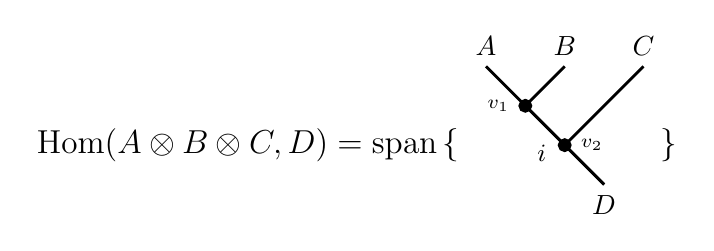
\begin{tikzpicture}[line width=1pt, node distance=1cm]

    \node at (-1.5, 1) {\large $\mathrm{Hom}(A \otimes B \otimes C, D) = \mathrm{span} \left\{ \vphantom{\sum} \right.$};

    \begin{scope}[shift={(1.5,0)}]
        % Incoming leaves
        \coordinate (A) at (0,2);
        \coordinate (B) at (1,2);
        \coordinate (C) at (2,2);
        \coordinate (D) at (1.5,0.5);
        
        \coordinate (V1) at (0.5, 1.5); 
        \coordinate (V2) at (1.0, 1); % 
        
        \draw (A) -- (D);
        \draw (B) -- (V1);
        \draw (V1) -- (V2);
        \draw (C) -- (V2);
        \draw (V2) -- (D);

        \filldraw (V1) circle (2pt) node[left=2pt, font=\scriptsize] {$v_1$};
        \filldraw (V2) circle (2pt) node[right=2pt, font=\scriptsize] {$v_2$};

        \node[above] at (A) {$A$};
        \node[above] at (B) {$B$};
        \node[above] at (C) {$C$};
        \node[below] at (D) {$D$};
        
        \node[left, font=\small] at (0.9,0.9) {$i$};
    \end{scope}


    \node at (3.8, 1) {\large $\left. \vphantom{\sum} \right\}$};

\end{tikzpicture}


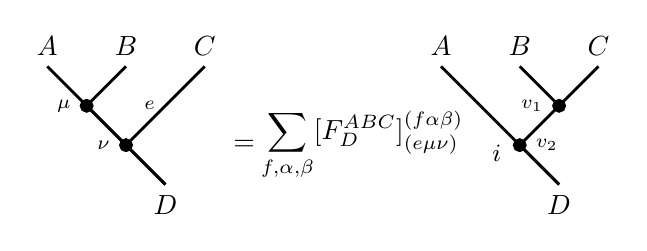
\begin{tikzpicture}[line width=1pt, node distance=1cm]

        % Incoming leaves
        \coordinate (A) at (0,2);
        \coordinate (B) at (1,2);
        \coordinate (C) at (2,2);
        \coordinate (D) at (1.5,0.5);
        
        \coordinate (V1) at (0.5, 1.5); 
        \coordinate (V2) at (1.0, 1); % 
        
        \draw (A) -- (D);
        \draw (B) -- (V1);
        \draw (V1) -- (V2);
        \draw (C) -- (V2);
        \draw (V2) -- (D);

        \filldraw (V1) circle (2pt) node[left=2pt, font=\scriptsize] {$\mu$};
        \filldraw (V2) circle (2pt) node[left=2pt, font=\scriptsize] {$\nu$};

        \node[above] at (A) {$A$};
        \node[above] at (B) {$B$};
        \node[above] at (C) {$C$};
        \node[below] at (D) {$D$};
        
        \node[left, font=\scriptsize] at (1.5,1.5) {$e$};
        \node at (2.5,1) {$=$};
        \node at (4,1) {$\displaystyle\sum_{f,\alpha,\beta} [F^{ABC}_{D}]_{(e \mu \nu)}^{(f \alpha \beta)} $};

        \begin{scope}[shift={(5,0)}]
        % Incoming leaves
        \coordinate (A) at (0,2);
        \coordinate (B) at (1,2);
        \coordinate (C) at (2,2);
        \coordinate (D) at (1.5,0.5);
        
        \coordinate (V2) at (1.0, 1); 
        \coordinate (V1) at (1.5, 1.5); % 
        
        \draw (A) -- (D);
        \draw (B) -- (V1);
        \draw (V1) -- (V2);
        \draw (C) -- (V1);
        \draw (V2) -- (D);

        \filldraw (V1) circle (2pt) node[left=2pt, font=\scriptsize] {$v_1$};
        \filldraw (V2) circle (2pt) node[right=2pt, font=\scriptsize] {$v_2$};

        \node[above] at (A) {$A$};
        \node[above] at (B) {$B$};
        \node[above] at (C) {$C$};
        \node[below] at (D) {$D$};
        
        \node[left, font=\small] at (0.9,0.9) {$i$};
    \end{scope}

\end{tikzpicture}


\begin{tikzpicture}
    
\end{tikzpicture}
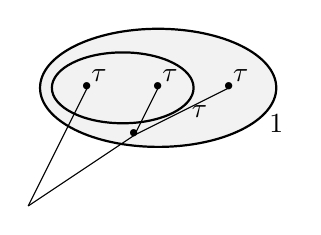
\begin{tikzpicture}[scale=1.5]

    \fill[gray!10] (3,0) ellipse (1 and 0.5);
    \draw[thick] (3,0) ellipse (1 and 0.5);
    
    \draw[thick] (2.7,0) ellipse (0.6 and 0.3);
    \node at (3.35,-0.2) {$\tau$};
    \node[scale=2.5] at (2.4, 0) {$\cdot$};
    \node at (2.5, 0.1) {$\tau$};
    \node[scale=2.5] at (3.0, 0) {$\cdot$};
    \node at (3.1,0.1) {$\tau$};
    \node[scale=2.5] at (3.6, 0) {$\cdot$};
    \node at (3.7,0.1) {$\tau$};
    \node at (4.0,-0.3) {$1$};
    \node[scale=2.5] at (2.8, -0.4) {$\cdot$};
    \draw (3.0, 0.0) -- (2.8, -0.4);
    \draw (3.6, 0.0) -- (2.8, -0.4); 
    \draw (2.8, -0.4) -- (1.9, -1.0);
    \draw (2.4, 0.0) -- (1.9, -1.0);
\end{tikzpicture}

% https://q.uiver.app/#q=WzAsMTQsWzAsMCwiKEFcXG90aW1lcyBCKVxcb3RpbWVzIEMiXSxbMiwwLCJBIFxcb3RpbWVzIChCIFxcb3RpbWVzIEMpIl0sWzAsMiwiSG9tKChBXFxvdGltZXMgQikgXFxvdGltZXMgQywgRCkiXSxbMiwyLCJIb20oQVxcb3RpbWVzIChCIFxcb3RpbWVzIEMpLCBEKSJdLFswLDUsIlxcZGlzcGxheXN0eWxlXFxiaWdvcGx1c19jIFZee0FCfV9jIFxcb3RpbWVzIFZee2NDfV9EIl0sWzIsNSwiXFxkaXNwbGF5c3R5bGVcXGJpZ29wbHVzX2MgVl57QWN9X0QgXFxvdGltZXMgVl57QkN9X2MiXSxbMSwyLCJcXGNvbmciXSxbMSw0LCJcXGNvbmciXSxbMCw2LCJcXHZlcnQgKEEsQik7YztcXG11XFxyYW5nbGUgXFxvdGltZXMgXFx2ZXJ0IGMsQzsgRDsgXFxudSBcXHJhbmdsZSJdLFsyLDYsIlxcc3VtX3tmLFxcYWxwaGEsXFxiZXRhfSBbRl9EXntBQkN9XV97KGNcXG11XFxudSl9XnsoZlxcYWxwaGFcXGJldGEpfSBcXHZlcnQgQSxmO0Q7XFxiZXRhXFxyYW5nbGUgXFxvdGltZXMgXFx2ZXJ0IEIsQzsgZjsgXFxhbHBoYSBcXHJhbmdsZSJdLFsxLDUsIlxcdGV4dHtjaG9pY2Ugb2YgYmFzaXN9Il0sWzAsNCwiXFxkaXNwbGF5c3R5bGVcXGJpZ29wbHVzX2MgSG9tKEEgXFxvdGltZXMgQiwgYykgXFxvdGltZXMgSG9tKGMgXFxvdGltZXMgQywgRCkiXSxbMiw0LCJcXGRpc3BsYXlzdHlsZVxcYmlnb3BsdXNfe2QgXFxpbiBJcnIoXFxtYXRoc2Z7Q2F0fSl9IEhvbShBIFxcb3RpbWVzIGQsIEQpIFxcb3RpbWVzIEhvbShCIFxcb3RpbWVzIEMsIGQpIl0sWzEsMywiXFx0ZXh0e3NlbWlzaW1wbGljaXR5fSJdLFswLDIsIkhvbSgtLEQpIiwxXSxbMSwzLCJIb20oLSxEKSIsMV0sWzAsMSwiXFxhbHBoYV97QUJDfSJdLFs0LDgsIlxcaW4iLDMseyJzdHlsZSI6eyJib2R5Ijp7Im5hbWUiOiJub25lIn0sImhlYWQiOnsibmFtZSI6Im5vbmUifX19XSxbOCw5LCIiLDEseyJsZXZlbCI6Miwic3R5bGUiOnsiaGVhZCI6eyJuYW1lIjoibm9uZSJ9fX1dLFsyLDExLCJcXHVuZGVyc2V0e1xcdGV4dHtzZW1pc2ltcGxpY2l0eX19e1xcY29uZ30iLDMseyJzdHlsZSI6eyJib2R5Ijp7Im5hbWUiOiJub25lIn0sImhlYWQiOnsibmFtZSI6Im5vbmUifX19XSxbMywxMiwiXFx1bmRlcnNldHtcXHRleHR7c2VtaXNpbXBsaWNpdHl9fXtcXGNvbmd9IiwzLHsic3R5bGUiOnsiYm9keSI6eyJuYW1lIjoibm9uZSJ9LCJoZWFkIjp7Im5hbWUiOiJub25lIn19fV0sWzExLDQsIlxcY29uZyIsMyx7InN0eWxlIjp7ImJvZHkiOnsibmFtZSI6Im5vbmUifSwiaGVhZCI6eyJuYW1lIjoibm9uZSJ9fX1dLFsxMiw1LCJcXGNvbmciLDMseyJzdHlsZSI6eyJib2R5Ijp7Im5hbWUiOiJub25lIn0sImhlYWQiOnsibmFtZSI6Im5vbmUifX19XSxbNSw5LCJcXGluIiwzLHsic3R5bGUiOnsiYm9keSI6eyJuYW1lIjoibm9uZSJ9LCJoZWFkIjp7Im5hbWUiOiJub25lIn19fV0sWzE2LDYsIlxcdGV4dHtZb25lZGEtbGlmdGluZ30iLDEseyJzaG9ydGVuIjp7InNvdXJjZSI6MjB9LCJzdHlsZSI6eyJib2R5Ijp7Im5hbWUiOiJub25lIn0sImhlYWQiOnsibmFtZSI6Im5vbmUifX19XV0=
\[\begin{tikzcd}
	{(A\otimes B)\otimes C} && {A \otimes (B \otimes C)} \\
	\\
	{Hom((A\otimes B) \otimes C, D)} & \cong & {Hom(A\otimes (B \otimes C), D)} \\
	& {\text{semisimplicity}} \\
	{\displaystyle\bigoplus_c Hom(A \otimes B, c) \otimes Hom(c \otimes C, D)} & \cong & {\displaystyle\bigoplus_{d \in Irr(\mathsf{Cat})} Hom(A \otimes d, D) \otimes Hom(B \otimes C, d)} \\
	{\displaystyle\bigoplus_c V^{AB}_c \otimes V^{cC}_D} & {\text{choice of basis}} & {\displaystyle\bigoplus_c V^{Ac}_D \otimes V^{BC}_c} \\
	{\vert (A,B);c;\mu\rangle \otimes \vert c,C; D; \nu \rangle} && {\sum_{f,\alpha,\beta} [F_D^{ABC}]_{(c\mu\nu)}^{(f\alpha\beta)} \vert A,f;D;\beta\rangle \otimes \vert B,C; f; \alpha \rangle}
	\arrow[""{name=0, anchor=center, inner sep=0}, "{\alpha_{ABC}}", from=1-1, to=1-3]
	\arrow["{Hom(-,D)}"{description}, from=1-1, to=3-1]
	\arrow["{Hom(-,D)}"{description}, from=1-3, to=3-3]
	\arrow["{\underset{\text{semisimplicity}}{\cong}}"{marking, allow upside down}, draw=none, from=3-1, to=5-1]
	\arrow["{\underset{\text{semisimplicity}}{\cong}}"{marking, allow upside down}, draw=none, from=3-3, to=5-3]
	\arrow["\cong"{marking, allow upside down}, draw=none, from=5-1, to=6-1]
	\arrow["\cong"{marking, allow upside down}, draw=none, from=5-3, to=6-3]
	\arrow["\in"{marking, allow upside down}, draw=none, from=6-1, to=7-1]
	\arrow["\in"{marking, allow upside down}, draw=none, from=6-3, to=7-3]
	\arrow[equals, from=7-1, to=7-3]
	\arrow["{\text{Yoneda-lifting}}"{description}, draw=none, from=0, to=3-2]
\end{tikzcd}\]


Let $f : E \to A \otimes B$ and $g : D \to E \otimes C$.

%\newcommand{\blue}[1]{\textcolor{blue}{#1}}
%\newcommand{\green}[1]{\textcolor{green}{#1}}

% https://q.uiver.app/#q=WzAsMTIsWzAsMCwiKEFcXG90aW1lcyBCKVxcb3RpbWVzIEMiXSxbMiwwLCJBIFxcb3RpbWVzIChCIFxcb3RpbWVzIEMpIl0sWzAsMiwiSG9tKChBXFxvdGltZXMgQikgXFxvdGltZXMgQywgRCkiXSxbMiwyLCJIb20oQVxcb3RpbWVzIChCIFxcb3RpbWVzIEMpLCBEKSJdLFswLDUsIlxcZGlzcGxheXN0eWxlXFxiaWdvcGx1c19jIFZee0FCfV9jIFxcb3RpbWVzIFZee2NDfV9EIl0sWzIsNSwiXFxkaXNwbGF5c3R5bGVcXGJpZ29wbHVzX2MgVl57QWN9X0QgXFxvdGltZXMgVl57QkN9X2MiXSxbMSw0LCJcXGNvbmciXSxbMCw2LCJcXHVuZGVyc2V0e1xcYmx1ZXtcXG11IFxcaW4gMSxcXGxkb3RzLCBOXntBQn1fY30gXFxxdWFkIFxcYmx1ZXtcXG51IFxcaW4gMSxcXGxkb3RzLE5ee2NDLER9fX17XFx2ZXJ0IChBLEIpO2M7XFxtdVxccmFuZ2xlIFxcb3RpbWVzIFxcdmVydCBjLEM7IEQ7IFxcbnUgXFxyYW5nbGV9Il0sWzIsNiwiXFxkaXNwbGF5c3R5bGVcXHN1bV97ZixcXGFscGhhLFxcYmV0YX0gW0ZfRF57QUJDfV1feyhjXFxtdVxcbnUpfV57KGZcXGFscGhhXFxiZXRhKX0gXFx2ZXJ0IEEsZjtEO1xcYmV0YVxccmFuZ2xlIFxcb3RpbWVzIFxcdmVydCBCLEM7IGY7IFxcYWxwaGEgXFxyYW5nbGUiXSxbMCw0LCJcXGRpc3BsYXlzdHlsZVxcYmlnb3BsdXNfe2NcXGluIElycihDQVQpfSBIb20oQSBcXG90aW1lcyBCLCBjKSBcXG90aW1lcyBIb20oYyBcXG90aW1lcyBDLCBEKSJdLFsyLDQsIlxcZGlzcGxheXN0eWxlXFxiaWdvcGx1c197ZCBcXGluIElycihcXG1hdGhzZntDYXR9KX0gSG9tKEEgXFxvdGltZXMgZCwgRCkgXFxvdGltZXMgSG9tKEIgXFxvdGltZXMgQywgZCkiXSxbMSw1LCJcXGNvbmciXSxbMCwyLCJIb20oLSxEKSIsMV0sWzEsMywiSG9tKC0sRCkiLDFdLFswLDEsIlxcdW5kZXJzZXR7XFxzaW19e1xcYWxwaGFfe0FCQ319Il0sWzQsNywiXFxpbiIsMyx7InN0eWxlIjp7ImJvZHkiOnsibmFtZSI6Im5vbmUifSwiaGVhZCI6eyJuYW1lIjoibm9uZSJ9fX1dLFs3LDgsIlxcdW5kZXJzZXR7XFxncmVlbntcXHRleHR7Nmotc3ltYm9sc319fXtGXntBQkN9X0R9IiwxLHsic2hvcnRlbiI6eyJzb3VyY2UiOjEwLCJ0YXJnZXQiOjEwfX1dLFsyLDksIlxcdW5kZXJzZXR7XFx0ZXh0e1xcZ3JlZW57c2VtaXNpbXBsaWNpdHl9fX17XFxjb25nfSIsMyx7InN0eWxlIjp7ImJvZHkiOnsibmFtZSI6Im5vbmUifSwiaGVhZCI6eyJuYW1lIjoibm9uZSJ9fX1dLFszLDEwLCJcXHVuZGVyc2V0e1xcdGV4dHtcXGdyZWVue3NlbWlzaW1wbGljaXR5fX19e1xcY29uZ30iLDMseyJvZmZzZXQiOi0yLCJzdHlsZSI6eyJib2R5Ijp7Im5hbWUiOiJub25lIn0sImhlYWQiOnsibmFtZSI6Im5vbmUifX19XSxbOSw0LCI9IiwzLHsic3R5bGUiOnsiYm9keSI6eyJuYW1lIjoibm9uZSJ9LCJoZWFkIjp7Im5hbWUiOiJub25lIn19fV0sWzEwLDUsIj0iLDMseyJzdHlsZSI6eyJib2R5Ijp7Im5hbWUiOiJub25lIn0sImhlYWQiOnsibmFtZSI6Im5vbmUifX19XSxbNSw4LCJcXGluIiwzLHsic3R5bGUiOnsiYm9keSI6eyJuYW1lIjoibm9uZSJ9LCJoZWFkIjp7Im5hbWUiOiJub25lIn19fV0sWzIsMywiXFx1bmRlcnNldHtcXHNpbX17XFxhbHBoYV97QSxCLEN9fSJdLFsyLDMsIlxcc21hbGxcXGdyZWVue1xcdGV4dHthc3NvY2lhdG9yIGluZHVjZXMgaXNvbW9ycGhpbXMgdW5kZXIgeW9uZWRhfX0iLDAseyJvZmZzZXQiOjUsInN0eWxlIjp7ImJvZHkiOnsibmFtZSI6Im5vbmUifSwiaGVhZCI6eyJuYW1lIjoibm9uZSJ9fX1dXQ==
\[\begin{tikzcd}
	{(A\otimes B)\otimes C} && {A \otimes (B \otimes C)} \\
	\\
	{Hom((A\otimes B) \otimes C, D)} && {Hom(A\otimes (B \otimes C), D)} \\
	\\
	{\displaystyle\bigoplus_{c\in Irr(CAT)} Hom(A \otimes B, c) \otimes Hom(c \otimes C, D)} & \cong & {\displaystyle\bigoplus_{d \in Irr(\mathsf{Cat})} Hom(A \otimes d, D) \otimes Hom(B \otimes C, d)} \\
	{\displaystyle\bigoplus_c V^{AB}_c \otimes V^{cC}_D} & \cong & {\displaystyle\bigoplus_c V^{Ac}_D \otimes V^{BC}_c} \\
	{\underset{\blue{\mu \in 1,\ldots, N^{AB}_c} \quad \blue{\nu \in 1,\ldots,N^{cC,D}}}{\vert (A,B);c;\mu\rangle \otimes \vert c,C; D; \nu \rangle}} && {\displaystyle\sum_{f,\alpha,\beta} [F_D^{ABC}]_{(c\mu\nu)}^{(f\alpha\beta)} \vert A,f;D;\beta\rangle \otimes \vert B,C; f; \alpha \rangle} \\
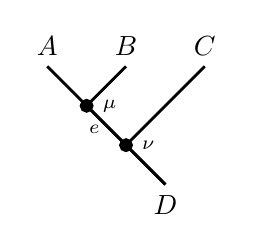
\begin{tikzpicture}[line width=1pt, node distance=1cm]
    % First diagram
    \coordinate (A) at (0,2);
    \coordinate (B) at (1,2);
    \coordinate (C) at (2,2);
    \coordinate (D) at (1.5,0.5);

    \coordinate (V1) at (0.5,1.5);
    \coordinate (V2) at (1.0,1);

    \draw (A) -- (D);
    \draw (B) -- (V1);
    \draw (V1) -- (V2);
    \draw (C) -- (V2);
    \draw (V2) -- (D);

    \filldraw (V1) circle (2pt) node[right=2pt,font=\scriptsize] {$\mu$};
    \filldraw (V2) circle (2pt) node[right=2pt,font=\scriptsize] {$\nu$};

    \node[above] at (A) {$A$};
    \node[above] at (B) {$B$};
    \node[above] at (C) {$C$};
    \node[below] at (D) {$D$};

    \node[left,font=\scriptsize] at (0.8,1.2) {$e$};
\end{tikzpicture}
&&
\hspace{-1.8cm}%
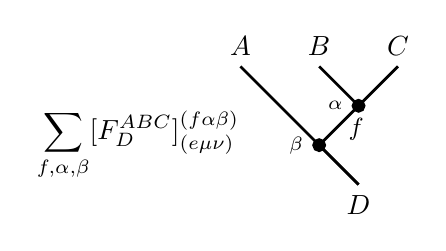
\begin{tikzpicture}[line width=1pt, node distance=1cm, xshift=-2cm]
    \begin{scope}[xshift=-2]
        
    \node at (-1.3,1) 
    {$\displaystyle\sum_{f,\alpha,\beta}
    [F^{ABC}_{D}]_{(e\mu\nu)}^{(f\alpha\beta)}$};

    \coordinate (A) at (0,2);
    \coordinate (B) at (1,2);
    \coordinate (C) at (2,2);
    \coordinate (D) at (1.5,0.5);

    \coordinate (V2) at (1.0,1);
    \coordinate (V1) at (1.5,1.5);

    \draw (A) -- (D);
    \draw (B) -- (V1);
    \draw (V1) -- (V2);
    \draw (C) -- (V1);
    \draw (V2) -- (D);

    \filldraw (V1) circle (2pt) node[left=2pt,font=\scriptsize] {$\alpha$};
    \filldraw (V2) circle (2pt) node[left=2pt,font=\scriptsize] {$\beta$};

    \node[above] at (A) {$A$};
    \node[above] at (B) {$B$};
    \node[above] at (C) {$C$};
    \node[below] at (D) {$D$};

    \node[left,font=\small] at (1.7,1.2) {$f$};
    \end{scope}
\end{tikzpicture}
	\arrow["{\underset{\sim}{\alpha_{ABC}}}", from=1-1, to=1-3]
	\arrow["{Hom(-,D)}"{description}, from=1-1, to=3-1]
	\arrow["{Hom(-,D)}"{description}, from=1-3, to=3-3]
	\arrow["{\underset{\sim}{\alpha_{A,B,C}}}", from=3-1, to=3-3]
	\arrow["{\green{\text{associator induces isomorphims under yoneda}}}", shift right=5, draw=none, from=3-1, to=3-3]
	\arrow["{\underset{\text{\green{semisimplicity}}}{\cong}}"{marking, allow upside down}, draw=none, from=3-1, to=5-1]
	\arrow["{\underset{\text{\green{semisimplicity}}}{\cong}}"{marking, allow upside down}, shift left=2, draw=none, from=3-3, to=5-3]
	\arrow["{=}"{marking, allow upside down}, draw=none, from=5-1, to=6-1]
	\arrow["{=}"{marking, allow upside down}, draw=none, from=5-3, to=6-3]
	\arrow["\in"{marking, allow upside down}, draw=none, from=6-1, to=7-1]
	\arrow["\in"{marking, allow upside down}, draw=none, from=6-3, to=7-3]
	\arrow["{\underset{\green{\text{6j-symbols}}}{F^{ABC}_D}}"{description},  from=7-1, to=7-3]
    \arrow["{=}"{marking, allow upside down}, draw=none, from=8-1, to=8-3]
\end{tikzcd}\]

% https://q.uiver.app/#q=WzAsMTAsWzAsMCwiKEFcXG90aW1lcyBCKVxcb3RpbWVzIEMiXSxbMSwwLCJBIFxcb3RpbWVzIChCIFxcb3RpbWVzIEMpIl0sWzAsMiwiSG9tKChBXFxvdGltZXMgQikgXFxvdGltZXMgQywgRCkiXSxbMSwyLCJIb20oQVxcb3RpbWVzIChCIFxcb3RpbWVzIEMpLCBEKSJdLFswLDUsIlxcZGlzcGxheXN0eWxlXFxiaWdvcGx1c19lIFZee0FCfV9lIFxcb3RpbWVzIFZee2VDfV9EIl0sWzEsNSwiXFxkaXNwbGF5c3R5bGVcXGJpZ29wbHVzX2YgVl57QWZ9X0QgXFxvdGltZXMgVl57QkN9X2YiXSxbMCw2LCJcXHVuZGVyc2V0e1xcYmx1ZXtcXG11IFxcaW4gMSxcXGxkb3RzLCBOXntBQn1fZX0gXFxxdWFkIFxcYmx1ZXtcXG51IFxcaW4gMSxcXGxkb3RzLE5ee2VDLER9fX17XFx2ZXJ0IChBLEIpO2U7XFxtdVxccmFuZ2xlIFxcb3RpbWVzIFxcdmVydCBlLEM7IEQ7IFxcbnUgXFxyYW5nbGV9Il0sWzEsNiwiXFxkaXNwbGF5c3R5bGVcXHN1bV97ZixcXGFscGhhLFxcYmV0YX0gW0ZfRF57QUJDfV1feyhlXFxtdVxcbnUpfV57KGZcXGFscGhhXFxiZXRhKX0gXFx2ZXJ0IEEsZjtEO1xcYmV0YVxccmFuZ2xlIFxcb3RpbWVzIFxcdmVydCBCLEM7IGY7IFxcYWxwaGEgXFxyYW5nbGUiXSxbMCw0LCJcXGRpc3BsYXlzdHlsZVxcYmlnb3BsdXNfe2NcXGluIElycihDQVQpfSBIb20oQSBcXG90aW1lcyBCLCBjKSBcXG90aW1lcyBIb20oYyBcXG90aW1lcyBDLCBEKSJdLFsxLDQsIlxcZGlzcGxheXN0eWxlXFxiaWdvcGx1c197ZCBcXGluIElycihcXG1hdGhzZntDYXR9KX0gSG9tKEEgXFxvdGltZXMgZCwgRCkgXFxvdGltZXMgSG9tKEIgXFxvdGltZXMgQywgZCkiXSxbMCwyLCJIb20oLSxEKSIsMV0sWzEsMywiSG9tKC0sRCkiLDFdLFswLDEsIlxcdW5kZXJzZXR7XFxzaW19e1xcYWxwaGFfe0FCQ319Il0sWzQsNiwiXFxpbiIsMyx7InN0eWxlIjp7ImJvZHkiOnsibmFtZSI6Im5vbmUifSwiaGVhZCI6eyJuYW1lIjoibm9uZSJ9fX1dLFs2LDcsIlxcdW5kZXJzZXR7XFxncmVlbntcXHRleHR7Nmotc3ltYm9sc319fXtGXntBQkN9X0R9IiwxLHsic2hvcnRlbiI6eyJzb3VyY2UiOjEwLCJ0YXJnZXQiOjEwfX1dLFsyLDgsIlxcdW5kZXJzZXR7XFx0ZXh0e1xcZ3JlZW57c2VtaXNpbXBsaWNpdHl9fX17XFxjb25nfSIsMyx7InN0eWxlIjp7ImJvZHkiOnsibmFtZSI6Im5vbmUifSwiaGVhZCI6eyJuYW1lIjoibm9uZSJ9fX1dLFszLDksIlxcdW5kZXJzZXR7XFx0ZXh0e1xcZ3JlZW57c2VtaXNpbXBsaWNpdHl9fX17XFxjb25nfSIsMyx7Im9mZnNldCI6LTIsInN0eWxlIjp7ImJvZHkiOnsibmFtZSI6Im5vbmUifSwiaGVhZCI6eyJuYW1lIjoibm9uZSJ9fX1dLFs4LDQsIj0iLDMseyJzdHlsZSI6eyJib2R5Ijp7Im5hbWUiOiJub25lIn0sImhlYWQiOnsibmFtZSI6Im5vbmUifX19XSxbOSw1LCI9IiwzLHsic3R5bGUiOnsiYm9keSI6eyJuYW1lIjoibm9uZSJ9LCJoZWFkIjp7Im5hbWUiOiJub25lIn19fV0sWzUsNywiXFxpbiIsMyx7InN0eWxlIjp7ImJvZHkiOnsibmFtZSI6Im5vbmUifSwiaGVhZCI6eyJuYW1lIjoibm9uZSJ9fX1dLFsyLDMsIlxcdW5kZXJzZXR7XFxzaW19e1xcYWxwaGFfe0EsQixDfX0iXSxbMiwzLCJcXHNtYWxsXFxncmVlbntcXHRleHR7YXNzb2NpYXRvciBpbmR1Y2VzIGlzb21vcnBoaW1zIHVuZGVyIHlvbmVkYX19IiwwLHsib2Zmc2V0Ijo1LCJzdHlsZSI6eyJib2R5Ijp7Im5hbWUiOiJub25lIn0sImhlYWQiOnsibmFtZSI6Im5vbmUifX19XSxbOCw5LCJcXGNvbmciLDEseyJzdHlsZSI6eyJib2R5Ijp7Im5hbWUiOiJub25lIn0sImhlYWQiOnsibmFtZSI6Im5vbmUifX19XSxbNCw1LCJcXGNvbmciLDEseyJzdHlsZSI6eyJib2R5Ijp7Im5hbWUiOiJub25lIn0sImhlYWQiOnsibmFtZSI6Im5vbmUifX19XV0=
\begin{tikzcd}[column sep=large]
	{(A\otimes B)\otimes C} & {A \otimes (B \otimes C)} \\
	\\
	{Hom((A\otimes B) \otimes C, D)} & {Hom(A\otimes (B \otimes C), D)} \\
	\\
	{\displaystyle\bigoplus_{c\in Irr(CAT)} Hom(A \otimes B, c) \otimes Hom(c \otimes C, D)} & {\displaystyle\bigoplus_{d \in Irr(\mathsf{Cat})} Hom(A \otimes d, D) \otimes Hom(B \otimes C, d)} \\
	{\displaystyle\bigoplus_e V^{AB}_e \otimes V^{eC}_D} & {\displaystyle\bigoplus_f V^{Af}_D \otimes V^{BC}_f} \\
	{\underset{\blue{\mu \in 1,\ldots, N^{AB}_e} \quad \blue{\nu \in 1,\ldots,N^{eC,D}}}{\vert (A,B);e;\mu\rangle \otimes \vert e,C; D; \nu \rangle}} & {\displaystyle\sum_{f,\alpha,\beta} [F_D^{ABC}]_{(e\mu\nu)}^{(f\alpha\beta)} \vert A,f;D;\beta\rangle \otimes \vert B,C; f; \alpha \rangle}
	\arrow["{\underset{\sim}{\alpha_{ABC}}}", from=1-1, to=1-2]
	\arrow["{Hom(-,D)}"{description}, from=1-1, to=3-1]
	\arrow["{Hom(-,D)}"{description}, from=1-2, to=3-2]
	\arrow["{\underset{\sim}{\alpha_{A,B,C}}}", from=3-1, to=3-2]
	\arrow["{\green{\text{\small{associator induces isomorphims under yoneda}}}}", shift right=5, draw=none, from=3-1, to=3-2]
	\arrow["{\underset{\text{\green{semisimplicity}}}{\cong}}"{marking, allow upside down}, draw=none, from=3-1, to=5-1]
	\arrow["{\underset{\text{\green{semisimplicity}}}{\cong}}"{marking, allow upside down}, shift left=2, draw=none, from=3-2, to=5-2]
	\arrow["\cong"{description}, draw=none, from=5-1, to=5-2]
	\arrow["{=}"{marking, allow upside down}, draw=none, from=5-1, to=6-1]
	\arrow["{=}"{marking, allow upside down}, draw=none, from=5-2, to=6-2]
	\arrow["\cong"{description}, draw=none, from=6-1, to=6-2]
	\arrow["\in"{marking, allow upside down}, draw=none, from=6-1, to=7-1]
	\arrow["\in"{marking, allow upside down}, draw=none, from=6-2, to=7-2]
	\arrow["{\underset{\green{\text{6j-symbols}}}{F^{ABC}_D}}"{description}, from=7-1, to=7-2]
\end{tikzcd}



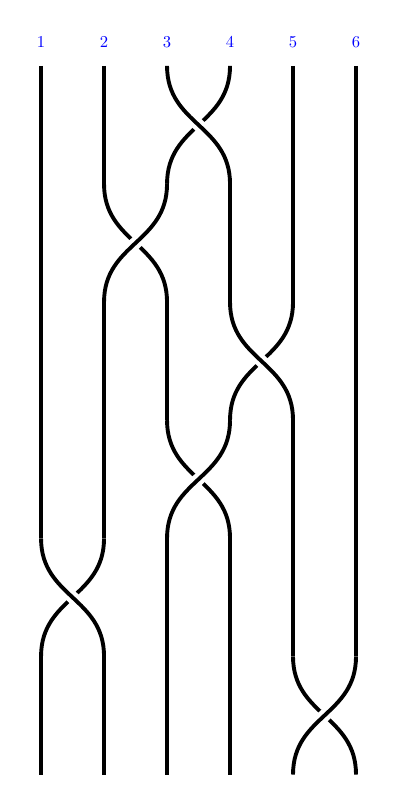
\begin{tikzpicture}[yscale=1.0]
  \draw (-2.00, 0.3) node {\color{blue}\scalebox{.6}{1}};
  \draw (-1.20, 0.3) node {\color{blue}\scalebox{.6}{2}};
  \draw (-0.40, 0.3) node {\color{blue}\scalebox{.6}{3}};
  \draw (0.40, 0.3) node {\color{blue}\scalebox{.6}{4}};
  \draw (1.20, 0.3) node {\color{blue}\scalebox{.6}{5}};
  \draw (2.00, 0.3) node {\color{blue}\scalebox{.6}{6}};
  \draw[line width=1.4] (-2.00, 0.00) to (-2.00, -1.50);
  \draw[line width=1.4] (-1.20, 0.00) to (-1.20, -1.50);
  \draw[line width=1.4] (1.20, 0.00) to (1.20, -1.50);
  \draw[line width=1.4] (2.00, 0.00) to (2.00, -1.50);
  \draw[line width=1.4] (0.40, 0.00) .. controls (0.40, -0.75) and (-0.40, -0.75) .. (-0.40, -1.50);
  \draw[line width=4.5, white] (-0.40, 0.00) .. controls (-0.40, -0.75) and (0.40, -0.75) .. (0.40, -1.50);
  \draw[line width=1.4] (-0.40, 0.00) .. controls (-0.40, -0.75) and (0.40, -0.75) .. (0.40, -1.50);
  \draw[line width=1.4] (-2.00, -1.50) to (-2.00, -3.00);
  \draw[line width=1.4] (0.40, -1.50) to (0.40, -3.00);
  \draw[line width=1.4] (1.20, -1.50) to (1.20, -3.00);
  \draw[line width=1.4] (2.00, -1.50) to (2.00, -3.00);
  \draw[line width=1.4] (-1.20, -1.50) .. controls (-1.20, -2.25) and (-0.40, -2.25) .. (-0.40, -3.00);
  \draw[line width=4.5, white] (-0.40, -1.50) .. controls (-0.40, -2.25) and (-1.20, -2.25) .. (-1.20, -3.00);
  \draw[line width=1.4] (-0.40, -1.50) .. controls (-0.40, -2.25) and (-1.20, -2.25) .. (-1.20, -3.00);
  \draw[line width=1.4] (-2.00, -3.00) to (-2.00, -4.50);
  \draw[line width=1.4] (-1.20, -3.00) to (-1.20, -4.50);
  \draw[line width=1.4] (-0.40, -3.00) to (-0.40, -4.50);
  \draw[line width=1.4] (2.00, -3.00) to (2.00, -4.50);
  \draw[line width=1.4] (1.20, -3.00) .. controls (1.20, -3.75) and (0.40, -3.75) .. (0.40, -4.50);
  \draw[line width=4.5, white] (0.40, -3.00) .. controls (0.40, -3.75) and (1.20, -3.75) .. (1.20, -4.50);
  \draw[line width=1.4] (0.40, -3.00) .. controls (0.40, -3.75) and (1.20, -3.75) .. (1.20, -4.50);
  \draw[line width=1.4] (-2.00, -4.50) to (-2.00, -6.00);
  \draw[line width=1.4] (-1.20, -4.50) to (-1.20, -6.00);
  \draw[line width=1.4] (1.20, -4.50) to (1.20, -6.00);
  \draw[line width=1.4] (2.00, -4.50) to (2.00, -6.00);
  \draw[line width=1.4] (-0.40, -4.50) .. controls (-0.40, -5.25) and (0.40, -5.25) .. (0.40, -6.00);
  \draw[line width=4.5, white] (0.40, -4.50) .. controls (0.40, -5.25) and (-0.40, -5.25) .. (-0.40, -6.00);
  \draw[line width=1.4] (0.40, -4.50) .. controls (0.40, -5.25) and (-0.40, -5.25) .. (-0.40, -6.00);
  \draw[line width=1.4] (-0.40, -6.00) to (-0.40, -7.50);
  \draw[line width=1.4] (0.40, -6.00) to (0.40, -7.50);
  \draw[line width=1.4] (1.20, -6.00) to (1.20, -7.50);
  \draw[line width=1.4] (2.00, -6.00) to (2.00, -7.50);
  \draw[line width=1.4] (-1.20, -6.00) .. controls (-1.20, -6.75) and (-2.00, -6.75) .. (-2.00, -7.50);
  \draw[line width=4.5, white] (-2.00, -6.00) .. controls (-2.00, -6.75) and (-1.20, -6.75) .. (-1.20, -7.50);
  \draw[line width=1.4] (-2.00, -6.00) .. controls (-2.00, -6.75) and (-1.20, -6.75) .. (-1.20, -7.50);
  \draw[line width=1.4] (-2.00, -7.50) to (-2.00, -9.00);
  \draw[line width=1.4] (-1.20, -7.50) to (-1.20, -9.00);
  \draw[line width=1.4] (-0.40, -7.50) to (-0.40, -9.00);
  \draw[line width=1.4] (0.40, -7.50) to (0.40, -9.00);
  \draw[line width=1.4] (1.20, -7.50) .. controls (1.20, -8.25) and (2.00, -8.25) .. (2.00, -9.00);
  \draw[line width=4.5, white] (2.00, -7.50) .. controls (2.00, -8.25) and (1.20, -8.25) .. (1.20, -9.00);
  \draw[line width=1.4] (2.00, -7.50) .. controls (2.00, -8.25) and (1.20, -8.25) .. (1.20, -9.00);
\end{tikzpicture}

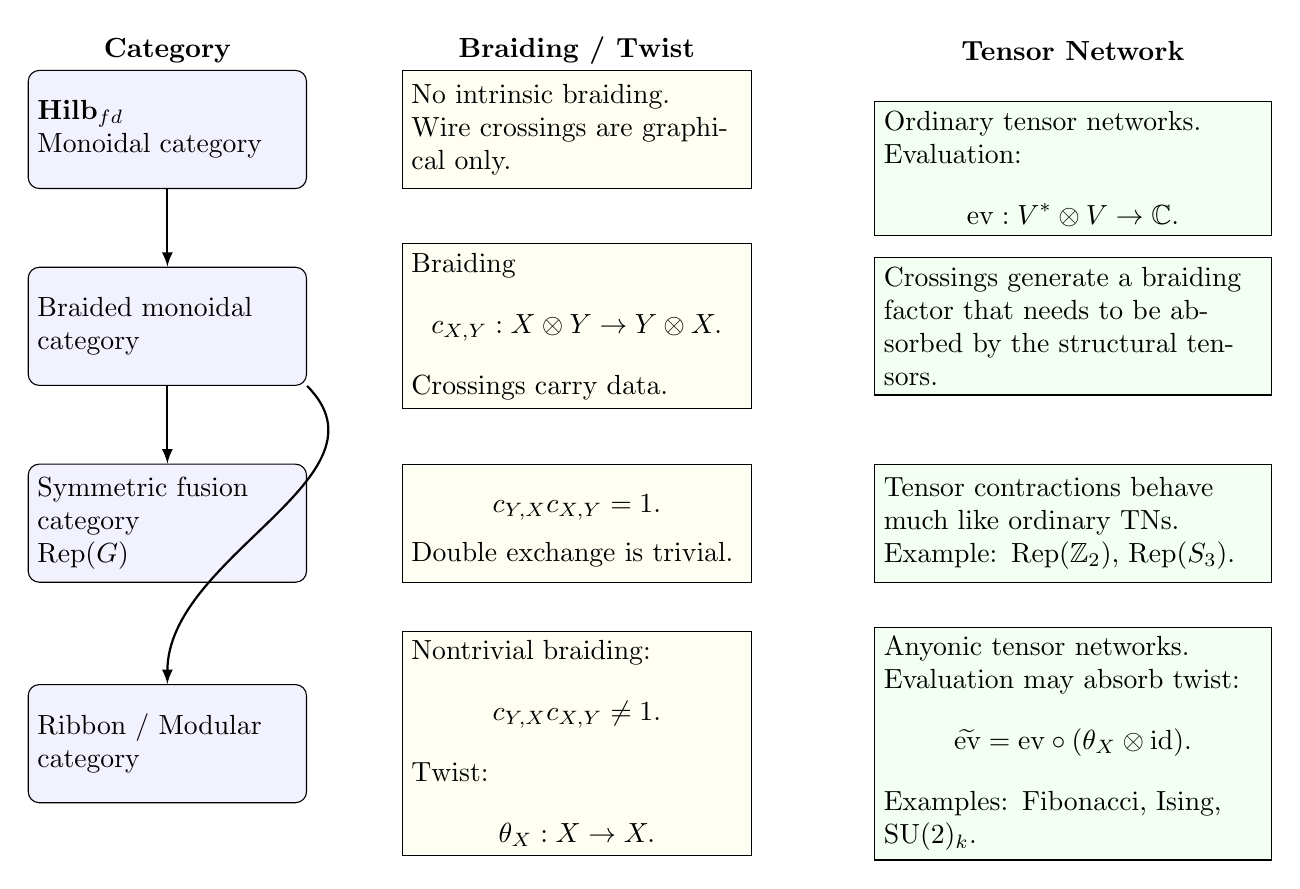
\begin{tikzpicture}[
  >=latex,
  cat/.style={
      draw,
      rounded corners,
      fill=blue!5,
      text width=3.3cm,
      align=left,
      minimum height=1.5cm
  },
  prop/.style={
      draw,
      fill=yellow!5,
      text width=4.2cm,
      align=left,
      minimum height=1.5cm
  },
  ex/.style={
      draw,
      fill=green!5,
      text width=4.8cm,
      align=left,
      minimum height=1.5cm
  }
]

\node[font=\bfseries] at (0,1) {Category};
\node[font=\bfseries] at (5.2,1) {Braiding / Twist};
\node[font=\bfseries] at (11.5,1) {Tensor Network};

\node[cat] (hilb) at (0,0)
{
$\mathbf{Hilb}_{fd}$\\
Monoidal category
};

\node[prop] (hilbp) at (5.2,0)
{
No intrinsic braiding.
Wire crossings are graphical only.
};

\node[ex] (hilbe) at (11.5,-0.5)
{
Ordinary tensor networks.\\
Evaluation:
\[
\mathrm{ev}:V^*\otimes V\to\mathbb C.
\]
};

\node[cat] (braid) at (0,-2.5)
{
Braided monoidal category
};

\node[prop] (braidp) at (5.2,-2.5)
{
Braiding
\[
c_{X,Y}:X\otimes Y\to Y\otimes X.
\]
Crossings carry data.
};

\node[ex] (braide) at (11.5,-2.5)
{
Crossings generate a braiding factor that needs to be absorbed by the structural tensors.
};

\node[cat] (symm) at (0,-5)
{
Symmetric fusion category\\
$\mathrm{Rep}(G)$
};

\node[prop] (symmp) at (5.2,-5)
{
\[
c_{Y,X}c_{X,Y}=1.
\]
Double exchange is trivial.
};

\node[ex] (symme) at (11.5,-5)
{
Tensor contractions behave much like ordinary TNs.

Example:
$\mathrm{Rep}(\mathbb Z_2)$,
$\mathrm{Rep}(S_3)$.
};

\node[cat] (mod) at (0,-7.8)
{
Ribbon / Modular category
};

\node[prop] (modp) at (5.2,-7.8)
{
Nontrivial braiding:
\[
c_{Y,X}c_{X,Y}\neq 1.
\]

Twist:
\[
\theta_X:X\to X.
\]
};

\node[ex] (mode) at (11.5,-7.8)
{
Anyonic tensor networks.

Evaluation may absorb twist:
\[
\widetilde{\mathrm{ev}}
=
\mathrm{ev}\circ
(\theta_X\otimes \mathrm{id}).
\]

Examples:
Fibonacci,
Ising,
$\mathrm{SU}(2)_k$.
};


\draw[->,thick] (hilb.south) -- (braid.north);
\draw[->,thick] (braid.south) -- (symm.north);

\draw[->,thick]
(braid.south east)
to[out=-45,in=90]
(mod.north);

\end{tikzpicture}

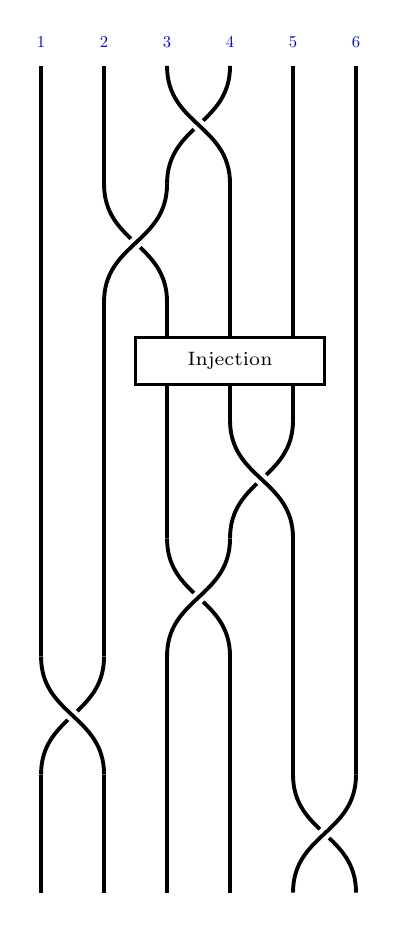
\begin{tikzpicture}[yscale=1.0]
  \draw (-2.00, 0.3) node {\color{blue}\scalebox{.6}{1}};
  \draw (-1.20, 0.3) node {\color{blue}\scalebox{.6}{2}};
  \draw (-0.40, 0.3) node {\color{blue}\scalebox{.6}{3}};
  \draw (0.40, 0.3) node {\color{blue}\scalebox{.6}{4}};
  \draw (1.20, 0.3) node {\color{blue}\scalebox{.6}{5}};
  \draw (2.00, 0.3) node {\color{blue}\scalebox{.6}{6}};
  \draw[line width=1.4] (-2.00, 0.00) to (-2.00, -1.50);
  \draw[line width=1.4] (-1.20, 0.00) to (-1.20, -1.50);
  \draw[line width=1.4] (1.20, 0.00) to (1.20, -1.50);
  \draw[line width=1.4] (2.00, 0.00) to (2.00, -1.50);
  \draw[line width=1.4] (0.40, 0.00) .. controls (0.40, -0.75) and (-0.40, -0.75) .. (-0.40, -1.50);
  \draw[line width=4.5, white] (-0.40, 0.00) .. controls (-0.40, -0.75) and (0.40, -0.75) .. (0.40, -1.50);
  \draw[line width=1.4] (-0.40, 0.00) .. controls (-0.40, -0.75) and (0.40, -0.75) .. (0.40, -1.50);
  \draw[line width=1.4] (-2.00, -1.50) to (-2.00, -3.00);
  \draw[line width=1.4] (0.40, -1.50) to (0.40, -3.00);
  \draw[line width=1.4] (1.20, -1.50) to (1.20, -3.00);
  \draw[line width=1.4] (2.00, -1.50) to (2.00, -3.00);
  \draw[line width=1.4] (-1.20, -1.50) .. controls (-1.20, -2.25) and (-0.40, -2.25) .. (-0.40, -3.00);
  \draw[line width=4.5, white] (-0.40, -1.50) .. controls (-0.40, -2.25) and (-1.20, -2.25) .. (-1.20, -3.00);
  \draw[line width=1.4] (-0.40, -1.50) .. controls (-0.40, -2.25) and (-1.20, -2.25) .. (-1.20, -3.00);
  \draw[line width=1.4] (-2.00, -3.00) to (-2.00, -4.50);
  \draw[line width=1.4] (-1.20, -3.00) to (-1.20, -4.50);
  \draw[line width=1.4] (2.00, -3.00) to (2.00, -4.50);
  \draw[line width=1.4] (-0.40, -3.00) to (-0.40, -3.45);
  \draw[line width=1.4] (0.40, -3.00) to (0.40, -3.45);
  \draw[line width=1.4] (1.20, -3.00) to (1.20, -3.45);
  \filldraw[fill=white, draw=black, line width=1.2] (-0.80, -3.45) rectangle (1.60, -4.05);
  \node at (0.40, -3.75) {\scriptsize Injection};
  \draw[line width=1.4] (-0.40, -4.05) to (-0.40, -4.50);
  \draw[line width=1.4] (0.40, -4.05) to (0.40, -4.50);
  \draw[line width=1.4] (1.20, -4.05) to (1.20, -4.50);
  \draw[line width=1.4] (-2.00, -4.50) to (-2.00, -6.00);
  \draw[line width=1.4] (-1.20, -4.50) to (-1.20, -6.00);
  \draw[line width=1.4] (-0.40, -4.50) to (-0.40, -6.00);
  \draw[line width=1.4] (2.00, -4.50) to (2.00, -6.00);
  \draw[line width=1.4] (1.20, -4.50) .. controls (1.20, -5.25) and (0.40, -5.25) .. (0.40, -6.00);
  \draw[line width=4.5, white] (0.40, -4.50) .. controls (0.40, -5.25) and (1.20, -5.25) .. (1.20, -6.00);
  \draw[line width=1.4] (0.40, -4.50) .. controls (0.40, -5.25) and (1.20, -5.25) .. (1.20, -6.00);
  \draw[line width=1.4] (-2.00, -6.00) to (-2.00, -7.50);
  \draw[line width=1.4] (-1.20, -6.00) to (-1.20, -7.50);
  \draw[line width=1.4] (1.20, -6.00) to (1.20, -7.50);
  \draw[line width=1.4] (2.00, -6.00) to (2.00, -7.50);
  \draw[line width=1.4] (-0.40, -6.00) .. controls (-0.40, -6.75) and (0.40, -6.75) .. (0.40, -7.50);
  \draw[line width=4.5, white] (0.40, -6.00) .. controls (0.40, -6.75) and (-0.40, -6.75) .. (-0.40, -7.50);
  \draw[line width=1.4] (0.40, -6.00) .. controls (0.40, -6.75) and (-0.40, -6.75) .. (-0.40, -7.50);
  \draw[line width=1.4] (-0.40, -7.50) to (-0.40, -9.00);
  \draw[line width=1.4] (0.40, -7.50) to (0.40, -9.00);
  \draw[line width=1.4] (1.20, -7.50) to (1.20, -9.00);
  \draw[line width=1.4] (2.00, -7.50) to (2.00, -9.00);
  \draw[line width=1.4] (-1.20, -7.50) .. controls (-1.20, -8.25) and (-2.00, -8.25) .. (-2.00, -9.00);
  \draw[line width=4.5, white] (-2.00, -7.50) .. controls (-2.00, -8.25) and (-1.20, -8.25) .. (-1.20, -9.00);
  \draw[line width=1.4] (-2.00, -7.50) .. controls (-2.00, -8.25) and (-1.20, -8.25) .. (-1.20, -9.00);
  \draw[line width=1.4] (-2.00, -9.00) to (-2.00, -10.50);
  \draw[line width=1.4] (-1.20, -9.00) to (-1.20, -10.50);
  \draw[line width=1.4] (-0.40, -9.00) to (-0.40, -10.50);
  \draw[line width=1.4] (0.40, -9.00) to (0.40, -10.50);
  \draw[line width=1.4] (1.20, -9.00) .. controls (1.20, -9.75) and (2.00, -9.75) .. (2.00, -10.50);
  \draw[line width=4.5, white] (2.00, -9.00) .. controls (2.00, -9.75) and (1.20, -9.75) .. (1.20, -10.50);
  \draw[line width=1.4] (2.00, -9.00) .. controls (2.00, -9.75) and (1.20, -9.75) .. (1.20, -10.50);
\end{tikzpicture}

%\[
%H_i = -J \begin{array}{r@{\hspace{0.00em}}c}
%  & \begin{array}{ccccc} \ket{1\tau 1} & \ket{\tau\tau 1} & \ket{1\tau\tau} & \ket{\tau 1 \tau} & \ket{\tau \tau, \tau} \end{array} \\
%  \begin{array}{r} \ket{1\tau 1} \\ \ket{\tau \tau 1} \\ \ket{1 \tau \tau} \\ \ket{\tau 1 \tau} \\ \ket{\tau \tau \tau} \end{array} & 
%  \begin{pmatrix}
%    1 &   &   &               &               \\
%      & 0 &   &               &               \\
%      &   & 0 &               &               \\
%      &   &   & \varphi^{-2}  & \varphi^{-\frac{3}{2}} \\
%      &   &   & \varphi^{-\frac{3}{2}} & \varphi^{-1}   \\
%  \end{pmatrix}
%\end{array}
%\]
%
%\[
%H_i = -J \begin{array}{r ccccc}
%  & \rotatebox{-90}{\,\ket{1\tau 1}} & \rotatebox{-90}{\,\ket{\tau\tau 1}} & \rotatebox{-90}{\,\ket{1\tau\tau}} & \rotatebox{-90}{\,\ket{\tau 1 \tau}} & \rotatebox{-90}{\,\ket{\tau \tau \tau}} \\
%  \begin{array}{r} \ket{1\tau 1} \\ \ket{\tau \tau 1} \\ \ket{1 \tau \tau} \\ \ket{\tau 1 \tau} \\ \ket{\tau \tau \tau} \end{array} & 
%  \multicolumn{5}{c}{
%    \begin{pmatrix}
%      1 & 0 & 0 & 0 & 0 \\
%      0 & 0 & 0 & 0 & 0 \\
%      0 & 0 & 0 & 0 & 0 \\
%      0 & 0 & 0 & \varphi^{-2}  & \varphi^{-\frac{3}{2}} \\
%      0 & 0 & 0 & \varphi^{-\frac{3}{2}} & \varphi^{-1}   \\
%    \end{pmatrix}
%  }
%\end{array}
%\]

\usetikzlibrary{arrows.meta, calc, decorations.pathmorphing, positioning, patterns, shapes.geometric}

% ---------- style for a braid strand segment ----------
\tikzset{
  strand/.style   = {line width=1.4pt, line cap=round},
  gap/.style      = {white, line width=6pt, line cap=butt},
  fiberline/.style= {blue!55!black, line width=0.9pt},
  basepath/.style = {->, thick, decorate, decoration={snake, amplitude=0.4mm, segment length=2.2mm, post length=1mm}}
}

% Draws one crossing level between positions p and p+1, from height y0 to y0+1,
% with strand of color cOver going OVER strand of color cUnder.
% "dir=lr" means the over-strand goes from left(p) to right(p+1) on top;
% "dir=rl" means the over-strand goes from right(p+1) to left(p) on top.
\newcommand{\crossing}[5]{%
  % #1=p (left x at y0)   #2=y0   #3=cOver  #4=cUnder  #5=dir (lr or rl)
  \def\p{#1}\def\yz{#2}
  \pgfmathsetmacro{\pone}{\p+1}
  \pgfmathsetmacro{\ymid}{\yz+0.5}
  \pgfmathsetmacro{\xmid}{\p+0.5}
  \ifx#5lr
    % under strand: from (p+1,y0) to (p,y0+1)
    \draw[strand, #4] (\pone,\yz) -- (\p,\yz+1);
    \draw[gap, rotate around={45:(\xmid,\ymid)}] (\xmid-0.28,\ymid) -- (\xmid+0.28,\ymid);
    \draw[strand, #3] (\p,\yz) -- (\pone,\yz+1);
  \else
    % under strand: from (p,y0) to (p+1,y0+1)
    \draw[strand, #4] (\p,\yz) -- (\pone,\yz+1);
    \draw[gap, rotate around={-45:(\xmid,\ymid)}] (\xmid-0.28,\ymid) -- (\xmid+0.28,\ymid);
    \draw[strand, #3] (\pone,\yz) -- (\p,\yz+1);
  \fi
}

\begin{tikzpicture}[>=Stealth]

%=====================================================================
% PANEL 1 (bottom): explicit braid of n=4 particles in the plane
%=====================================================================
\begin{scope}[local bounding box=braidpanel]

  \def\cA{red!70!black}
  \def\cB{blue!65!black}
  \def\cC{green!45!black}
  \def\cD{orange!85!black}

  % level 0->1 : cross positions 1,2  (A over B)
  \crossing{1}{0}{\cA}{\cB}{lr}
  \draw[strand,\cC] (3,0)--(3,1);
  \draw[strand,\cD] (4,0)--(4,1);

  % level 1->2 : cross positions 3,4  (C over D)
  \draw[strand,\cB] (1,1)--(1,2);
  \draw[strand,\cA] (2,1)--(2,2);
  \crossing{3}{1}{\cC}{\cD}{lr}

  % level 2->3 : cross positions 2,3  (A over D)
  \draw[strand,\cB] (1,2)--(1,3);
  \crossing{2}{2}{\cA}{\cD}{lr}
  \draw[strand,\cC] (4,2)--(4,3);

  % level 3->4 : cross positions 1,2  (B over D)
  \crossing{1}{3}{\cB}{\cD}{lr}
  \draw[strand,\cA] (3,3)--(3,4);
  \draw[strand,\cC] (4,3)--(4,4);

  % dots for the two configurations (t=0 bottom, t=1 top)
  \foreach \x/\c in {1/\cA,2/\cB,3/\cC,4/\cD}{
    \filldraw[\c] (\x,0) circle (2.6pt);
  }
  \foreach \x/\c in {1/\cD,2/\cB,3/\cA,4/\cC}{
    \filldraw[\c] (\x,4) circle (2.6pt);
  }

  \node[below] at (2.5,-0.35) {$q_0=\{z_1,\dots,z_4\}$, \; $t=0$};
  \node[above] at (2.5,4.35) {$q_1 = \beta\cdot q_0$, \; $t=1$};
  \node[right] at (4.6,2) {$\beta=\sigma_1\sigma_3\sigma_2\sigma_1 \in B_4$};

\end{scope}

%=====================================================================
% PANEL 2 (middle): the same braid as a loop/path in configuration space
%=====================================================================
\begin{scope}[yshift=6.6cm]

  \draw[thick, fill=gray!6] (2.5,0) ellipse (4.6 and 1.3);
  \node[below] at (2.5,-1.6) {$\mathrm{Conf}_4(\mathbb{R}^2)/S_4$};

  \coordinate (q0) at (0.6,0);
  \coordinate (q1) at (4.4,0);
  \filldraw[black] (q0) circle (2pt) node[below left=1pt] {$q_0$};
  \filldraw[black] (q1) circle (2pt) node[below right=1pt] {$q_1$};

  \draw[basepath] (q0) to[out=70,in=110] node[above]{$\gamma_\beta$} (q1);

  \draw[->, dashed, gray] (2.5,-1.35) -- (2.5,-2.9)
        node[midway,right,black,align=left]{\footnotesize the braid diagram below\\ \footnotesize \emph{is} a representative path $\gamma_\beta$\\ \footnotesize with $[\gamma_\beta]=\beta\in\pi_1\big(\mathrm{Conf}_4(\mathbb{R}^2)/S_4\big)$};

\end{scope}

%=====================================================================
% PANEL 3 (top): Hilbert bundle over configuration space
%=====================================================================
\begin{scope}[yshift=12.6cm]

  \draw[thick, fill=gray!6] (2.5,0) ellipse (4.6 and 1.3);
  \node[below] at (2.5,-1.6) {$\mathrm{Conf}_4(\mathbb{R}^2)/S_4$};

  \coordinate (q0) at (0.6,0);
  \coordinate (q1) at (4.4,0);
  \filldraw[black] (q0) circle (2pt) node[below] {$q_0$};
  \filldraw[black] (q1) circle (2pt) node[below] {$q_1$};

  % generic fibers
  \foreach \x in {-1.5,-0.4,1.6,2.6,3.6,5.6,6.6}{
    \draw[fiberline] (\x,0) -- (\x,2.1);
    \draw[fiberline] (\x,2.1) ellipse (0.22 and 0.09);
  }

  % highlighted fibers over q0, q1
  \draw[strand, violet!70!black] (0.6,0) -- (0.6,2.6);
  \draw[violet!70!black, fill=violet!10] (0.6,2.6) ellipse (0.32 and 0.13);
  \node[left] at (0.35,2.6) {$\mathcal{H}_{q_0}$};

  \draw[strand, teal!70!black] (4.4,0) -- (4.4,2.6);
  \draw[teal!70!black, fill=teal!10] (4.4,2.6) ellipse (0.32 and 0.13);
  \node[right] at (4.7,2.6) {$\mathcal{H}_{q_1}$};

  % monodromy / parallel transport arrow along the bundle
  \draw[->, thick, violet!40!teal] (0.9,2.65) to[out=25,in=155] node[above]{$\rho(\beta)$} (4.05,2.65);

  \node[above] at (2.5,3.25) {Hilbert bundle $\ \mathcal{H} \xrightarrow{\ \pi\ } \mathrm{Conf}_4(\mathbb{R}^2)/S_4$};
  \node[align=center] at (7.9,1.2) {\footnotesize parallel transport along\\ \footnotesize $\gamma_\beta$ gives the\\ \footnotesize monodromy / braid\\ \footnotesize representation\\ \footnotesize $\rho:B_4\to U(\mathcal{H})$};

  \draw[->,dashed,gray] (2.5,-1.35) -- (2.5,-2.05);

\end{scope}

\end{tikzpicture}

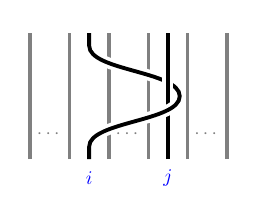
\begin{tikzpicture}[line width=1.2, yscale=.8]

\begin{scope}[shift={(-1,0)}, gray]
\draw (-.75,-1) to (-.75,1);
\draw (-.25,-1) to (-.25,1);
\draw (-.5,-.6) node {\scalebox{.7}{$\cdots$}};
\end{scope}


\begin{scope}[shift={(0,0)}, gray]
\draw (-.75,-1) to (-.75,1);
\draw (-.25,-1) to (-.25,1);
\draw (-.5,-.6) node {\scalebox{.7}{$\cdots$}};
\end{scope}

\draw[line width=1.4]
  (0,-1) to (0,1);

\begin{scope}[shift={(+1,0)}, gray]
\draw (-.75,-1) to (-.75,1);
\draw (-.25,-1) to (-.25,1);
\draw (-.5,-.6) node {\scalebox{.7}{$\cdots$}};
\end{scope}

\draw[line width=4pt, white]
  (-1, -1)
    --
  (-1, -.8)
    .. controls (-1,-.4) and (0.15, -.4) ..
  (0.15, 0)
    .. controls (0.15, +.4) and (-1, +.4) ..
  (-1,.8)
    --
  (-1,1);
\draw[line width=1.4]
  (-1, -1)
    --
  (-1, -.8)
    .. controls (-1,-.4) and (0.15, -.4) ..
  (0.15, 0)
    .. controls (0.15, +.4) and (-1, +.4) ..
  (-1,.8)
    --
  (-1,1);

\draw[line width=4, white]
  (0,0) to (0,1);
\draw[line width=1.4]
  (0,0) to (0,1);

\node
  at (-1,-1.3) {
    \scalebox{.7}{
      \color{blue}
      $i$
    }
  };

\node
  at (0,-1.3) {
    \scalebox{.7}{
      \color{blue}
      $j$
    }
  };

\end{tikzpicture}

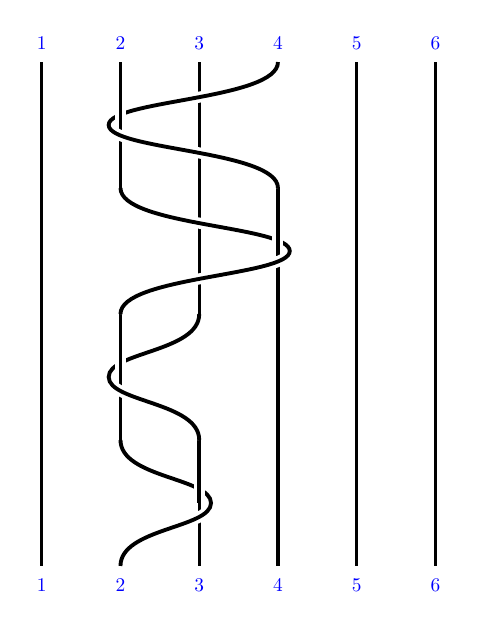
\begin{tikzpicture}[line width=1.2, yscale=.8]
% -- level 0: 2 over 3 --
\draw (0,-1) to (0,1);
\draw (3,-1) to (3,1);
\draw (4,-1) to (4,1);
\draw (5,-1) to (5,1);
\draw (2,-1) to (2,1);
\draw[line width=4pt, white] (1,-1) .. controls (1,-0.4) and (2.15,-0.4) .. (2.15,0) .. controls (2.15,0.4) and (1,0.4) .. (1,1);
\draw[line width=1.4] (1,-1) .. controls (1,-0.4) and (2.15,-0.4) .. (2.15,0) .. controls (2.15,0.4) and (1,0.4) .. (1,1);
\draw[line width=4pt, white] (2,0) to (2,1);
\draw[line width=1.4] (2,0) to (2,1);
% -- level 1: 3 over 2 --
\draw (0,1) to (0,3);
\draw (3,1) to (3,3);
\draw (4,1) to (4,3);
\draw (5,1) to (5,3);
\draw (1,1) to (1,3);
\draw[line width=4pt, white] (2,1) .. controls (2,1.6) and (0.85,1.6) .. (0.85,2) .. controls (0.85,2.4) and (2,2.4) .. (2,3);
\draw[line width=1.4] (2,1) .. controls (2,1.6) and (0.85,1.6) .. (0.85,2) .. controls (0.85,2.4) and (2,2.4) .. (2,3);
\draw[line width=4pt, white] (1,2) to (1,3);
\draw[line width=1.4] (1,2) to (1,3);
% -- level 2: 2 over 4 --
\draw (0,3) to (0,5);
\draw (2,3) to (2,5);
\draw (4,3) to (4,5);
\draw (5,3) to (5,5);
\draw (3,3) to (3,5);
\draw[line width=4pt, white] (1,3) .. controls (1,3.6) and (3.15,3.6) .. (3.15,4) .. controls (3.15,4.4) and (1,4.4) .. (1,5);
\draw[line width=1.4] (1,3) .. controls (1,3.6) and (3.15,3.6) .. (3.15,4) .. controls (3.15,4.4) and (1,4.4) .. (1,5);
\draw[line width=4pt, white] (3,4) to (3,5);
\draw[line width=1.4] (3,4) to (3,5);
% -- level 3: 4 over 2 --
\draw (0,5) to (0,7);
\draw (2,5) to (2,7);
\draw (4,5) to (4,7);
\draw (5,5) to (5,7);
\draw (1,5) to (1,7);
\draw[line width=4pt, white] (3,5) .. controls (3,5.6) and (0.85,5.6) .. (0.85,6) .. controls (0.85,6.4) and (3,6.4) .. (3,7);
\draw[line width=1.4] (3,5) .. controls (3,5.6) and (0.85,5.6) .. (0.85,6) .. controls (0.85,6.4) and (3,6.4) .. (3,7);
\draw[line width=4pt, white] (1,6) to (1,7);
\draw[line width=1.4] (1,6) to (1,7);
\node at (0,-1.3) {\scalebox{.7}{\color{blue}$1$}};
\node at (0,7.3) {\scalebox{.7}{\color{blue}$1$}};
\node at (1,-1.3) {\scalebox{.7}{\color{blue}$2$}};
\node at (1,7.3) {\scalebox{.7}{\color{blue}$2$}};
\node at (2,-1.3) {\scalebox{.7}{\color{blue}$3$}};
\node at (2,7.3) {\scalebox{.7}{\color{blue}$3$}};
\node at (3,-1.3) {\scalebox{.7}{\color{blue}$4$}};
\node at (3,7.3) {\scalebox{.7}{\color{blue}$4$}};
\node at (4,-1.3) {\scalebox{.7}{\color{blue}$5$}};
\node at (4,7.3) {\scalebox{.7}{\color{blue}$5$}};
\node at (5,-1.3) {\scalebox{.7}{\color{blue}$6$}};
\node at (5,7.3) {\scalebox{.7}{\color{blue}$6$}};
\end{tikzpicture}

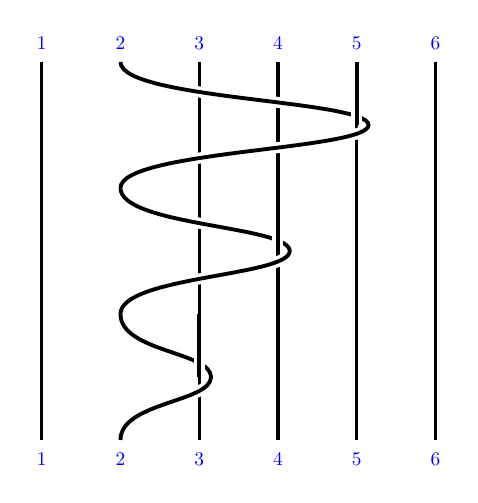
\begin{tikzpicture}[line width=1.2, yscale=.8]
% -- level 0: 2 over 3 --
\draw (0,-1) to (0,1);
\draw (3,-1) to (3,1);
\draw (4,-1) to (4,1);
\draw (5,-1) to (5,1);
\draw (2,-1) to (2,1);
\draw[line width=4pt, white] (1,-1) .. controls (1,-0.4) and (2.15,-0.4) .. (2.15,0) .. controls (2.15,0.4) and (1,0.4) .. (1,1);
\draw[line width=1.4] (1,-1) .. controls (1,-0.4) and (2.15,-0.4) .. (2.15,0) .. controls (2.15,0.4) and (1,0.4) .. (1,1);
\draw[line width=4pt, white] (2,0) to (2,1);
\draw[line width=1.4] (2,0) to (2,1);
% -- level 1: 2 over 4 --
\draw (0,1) to (0,3);
\draw (2,1) to (2,3);
\draw (4,1) to (4,3);
\draw (5,1) to (5,3);
\draw (3,1) to (3,3);
\draw[line width=4pt, white] (1,1) .. controls (1,1.6) and (3.15,1.6) .. (3.15,2) .. controls (3.15,2.4) and (1,2.4) .. (1,3);
\draw[line width=1.4] (1,1) .. controls (1,1.6) and (3.15,1.6) .. (3.15,2) .. controls (3.15,2.4) and (1,2.4) .. (1,3);
\draw[line width=4pt, white] (3,2) to (3,3);
\draw[line width=1.4] (3,2) to (3,3);
% -- level 2: 2 over 5 --
\draw (0,3) to (0,5);
\draw (2,3) to (2,5);
\draw (3,3) to (3,5);
\draw (5,3) to (5,5);
\draw (4,3) to (4,5);
\draw[line width=4pt, white] (1,3) .. controls (1,3.6) and (4.15,3.6) .. (4.15,4) .. controls (4.15,4.4) and (1,4.4) .. (1,5);
\draw[line width=1.4] (1,3) .. controls (1,3.6) and (4.15,3.6) .. (4.15,4) .. controls (4.15,4.4) and (1,4.4) .. (1,5);
\draw[line width=4pt, white] (4,4) to (4,5);
\draw[line width=1.4] (4,4) to (4,5);
\node at (0,-1.3) {\scalebox{.7}{\color{blue}$1$}};
\node at (0,5.3) {\scalebox{.7}{\color{blue}$1$}};
\node at (1,-1.3) {\scalebox{.7}{\color{blue}$2$}};
\node at (1,5.3) {\scalebox{.7}{\color{blue}$2$}};
\node at (2,-1.3) {\scalebox{.7}{\color{blue}$3$}};
\node at (2,5.3) {\scalebox{.7}{\color{blue}$3$}};
\node at (3,-1.3) {\scalebox{.7}{\color{blue}$4$}};
\node at (3,5.3) {\scalebox{.7}{\color{blue}$4$}};
\node at (4,-1.3) {\scalebox{.7}{\color{blue}$5$}};
\node at (4,5.3) {\scalebox{.7}{\color{blue}$5$}};
\node at (5,-1.3) {\scalebox{.7}{\color{blue}$6$}};
\node at (5,5.3) {\scalebox{.7}{\color{blue}$6$}};
\end{tikzpicture}

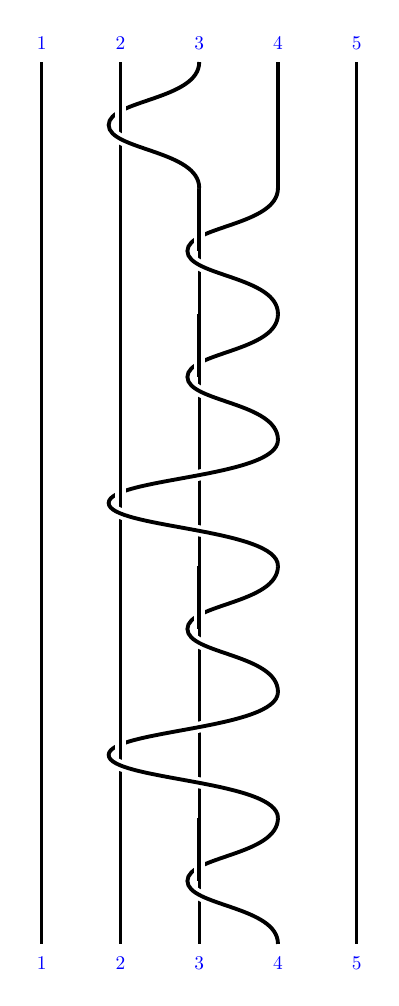
\begin{tikzpicture}[line width=1.2, yscale=.8]
% -- level 0: 4 over 3 --
\draw (0,-1) to (0,1);
\draw (1,-1) to (1,1);
\draw (4,-1) to (4,1);
\draw (2,-1) to (2,1);
\draw[line width=4pt, white] (3,-1) .. controls (3,-0.4) and (1.85,-0.4) .. (1.85,0) .. controls (1.85,0.4) and (3,0.4) .. (3,1);
\draw[line width=1.4] (3,-1) .. controls (3,-0.4) and (1.85,-0.4) .. (1.85,0) .. controls (1.85,0.4) and (3,0.4) .. (3,1);
\draw[line width=4pt, white] (2,0) to (2,1);
\draw[line width=1.4] (2,0) to (2,1);
% -- level 1: 4 over 2 --
\draw (0,1) to (0,3);
\draw (2,1) to (2,3);
\draw (4,1) to (4,3);
\draw (1,1) to (1,3);
\draw[line width=4pt, white] (3,1) .. controls (3,1.6) and (0.85,1.6) .. (0.85,2) .. controls (0.85,2.4) and (3,2.4) .. (3,3);
\draw[line width=1.4] (3,1) .. controls (3,1.6) and (0.85,1.6) .. (0.85,2) .. controls (0.85,2.4) and (3,2.4) .. (3,3);
\draw[line width=4pt, white] (1,2) to (1,3);
\draw[line width=1.4] (1,2) to (1,3);
% -- level 2: 4 over 3 --
\draw (0,3) to (0,5);
\draw (1,3) to (1,5);
\draw (4,3) to (4,5);
\draw (2,3) to (2,5);
\draw[line width=4pt, white] (3,3) .. controls (3,3.6) and (1.85,3.6) .. (1.85,4) .. controls (1.85,4.4) and (3,4.4) .. (3,5);
\draw[line width=1.4] (3,3) .. controls (3,3.6) and (1.85,3.6) .. (1.85,4) .. controls (1.85,4.4) and (3,4.4) .. (3,5);
\draw[line width=4pt, white] (2,4) to (2,5);
\draw[line width=1.4] (2,4) to (2,5);
% -- level 3: 4 over 2 --
\draw (0,5) to (0,7);
\draw (2,5) to (2,7);
\draw (4,5) to (4,7);
\draw (1,5) to (1,7);
\draw[line width=4pt, white] (3,5) .. controls (3,5.6) and (0.85,5.6) .. (0.85,6) .. controls (0.85,6.4) and (3,6.4) .. (3,7);
\draw[line width=1.4] (3,5) .. controls (3,5.6) and (0.85,5.6) .. (0.85,6) .. controls (0.85,6.4) and (3,6.4) .. (3,7);
\draw[line width=4pt, white] (1,6) to (1,7);
\draw[line width=1.4] (1,6) to (1,7);
% -- level 4: 4 over 3 --
\draw (0,7) to (0,9);
\draw (1,7) to (1,9);
\draw (4,7) to (4,9);
\draw (2,7) to (2,9);
\draw[line width=4pt, white] (3,7) .. controls (3,7.6) and (1.85,7.6) .. (1.85,8) .. controls (1.85,8.4) and (3,8.4) .. (3,9);
\draw[line width=1.4] (3,7) .. controls (3,7.6) and (1.85,7.6) .. (1.85,8) .. controls (1.85,8.4) and (3,8.4) .. (3,9);
\draw[line width=4pt, white] (2,8) to (2,9);
\draw[line width=1.4] (2,8) to (2,9);
% -- level 5: 4 over 3 --
\draw (0,9) to (0,11);
\draw (1,9) to (1,11);
\draw (4,9) to (4,11);
\draw (2,9) to (2,11);
\draw[line width=4pt, white] (3,9) .. controls (3,9.6) and (1.85,9.6) .. (1.85,10) .. controls (1.85,10.4) and (3,10.4) .. (3,11);
\draw[line width=1.4] (3,9) .. controls (3,9.6) and (1.85,9.6) .. (1.85,10) .. controls (1.85,10.4) and (3,10.4) .. (3,11);
\draw[line width=4pt, white] (2,10) to (2,11);
\draw[line width=1.4] (2,10) to (2,11);
% -- level 6: 3 over 2 --
\draw (0,11) to (0,13);
\draw (3,11) to (3,13);
\draw (4,11) to (4,13);
\draw (1,11) to (1,13);
\draw[line width=4pt, white] (2,11) .. controls (2,11.6) and (0.85,11.6) .. (0.85,12) .. controls (0.85,12.4) and (2,12.4) .. (2,13);
\draw[line width=1.4] (2,11) .. controls (2,11.6) and (0.85,11.6) .. (0.85,12) .. controls (0.85,12.4) and (2,12.4) .. (2,13);
\draw[line width=4pt, white] (1,12) to (1,13);
\draw[line width=1.4] (1,12) to (1,13);
\node at (0,-1.3) {\scalebox{.7}{\color{blue}$1$}};
\node at (0,13.3) {\scalebox{.7}{\color{blue}$1$}};
\node at (1,-1.3) {\scalebox{.7}{\color{blue}$2$}};
\node at (1,13.3) {\scalebox{.7}{\color{blue}$2$}};
\node at (2,-1.3) {\scalebox{.7}{\color{blue}$3$}};
\node at (2,13.3) {\scalebox{.7}{\color{blue}$3$}};
\node at (3,-1.3) {\scalebox{.7}{\color{blue}$4$}};
\node at (3,13.3) {\scalebox{.7}{\color{blue}$4$}};
\node at (4,-1.3) {\scalebox{.7}{\color{blue}$5$}};
\node at (4,13.3) {\scalebox{.7}{\color{blue}$5$}};
\end{tikzpicture}


% Source - https://tex.stackexchange.com/a/747428
% Posted by Urs Schreiber
% Retrieved 2026-09-22, License - CC BY-SA 4.0

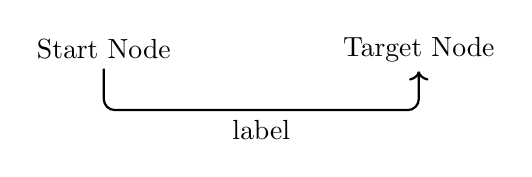
\begin{tikzpicture}
  \node (A) at (0,0) {Start Node};
  \node (B) at (4,0) {Target Node};

  \draw[->, thick] (A) to[u path] node[below] {label} (B);
\end{tikzpicture}

\end{document}